\documentclass[a4paper, 10pt]{article}
\usepackage{amsmath,amssymb,float,graphicx,pdfpages,titlesec,arydshln,hyperref}
\usepackage[utf8]{inputenc}
\usepackage[ngerman]{babel}
\usepackage[T1]{fontenc}
\usepackage[a4paper, left=2.5cm, top=3cm, bottom=2cm]{geometry}
\parindent0mm % if you want to have no lineskip
\parskip3mm


\begin{document}


\includepdf{interface18ws_titlepage}
\tableofcontents
\newpage
\section{Einleitung}
Um die Kommunikation sicherzustellen, hat das Interface Komitee dieses Dokument für
das Qwirkle-Projekt im Zuge des Software Praktikums im Wintersemester 2018/2019 entworfen.
Es hat das Ziel, die Kommunikation zwischen Server und Clients zu beschreiben.
So ermöglichen wir, dass diese Bestandteile unabhängig vom Entwickler korrekt
miteinander kommunizieren können.
\section{Glossar}
	\begin{itemize}
	\item Spieler: Spieler ist ein Client, der einem Spiel als Spieler beigetreten ist.
	\item Beobachter: Beobachter ist ein Client, mit ClientType Beobachter oder ein ClientType Player bzw. EnginePlayer der dem Game als Beobachter beigetreten ist. Ein Player oder EnginePlayer bleibt bis zum Ende des Games ein Beobachter.
	\item Client: Mit Client sind alle Clients gemeint, die mit dem gleichen Game verbunden sind. Unabhängig davon, ob es ein Spieler oder Beobachter ist.
	\item Lobby: Alle Clients landen nach dem Verbinden in der Lobby. Jeder Server hat genau eine Lobby. Eine Lobby hat beliebig viele Spiele.
	\item Spiel: Eine Spielsitzung in der Lobby eines Servers. Die Anzahl der Spieler wird in der Spielkonfiguration bestimmt. Es können beliebig viele Beobachter in einem Spiel sein.
	\item aktiver Spieler: Der aktive Spieler ist der Spieler eines Spiels, der momentan am Zug ist.
	\end{itemize}
\section{Verwendung}
Das Interface-Komitee stellt eine Implementierung, des in diesem Dokument definierten Interfaces, bereit. Dieses ist wie folgt zu benutzen:\\
Jeder Entwickler-Gruppe wird dieses Dokument, sowie die Interface-Library (.jar) mit der dazu gehörenden README.md, bereit gestellt. Wir empfehlen vor der Nutzung der Library dieses Dokument und die README gründlich zu lesen. Bei Fragen wenden Sie sich an das Komitee-Mitglied Ihrer Gruppe.\\
Die im Interface bereitgestellten Interface-Objekte werden mittels der Parser-Klasse in einen JSON-String umgewandelt. Dieser muss nun mittels einer selbst zu implementierenden Netzwerkverbindung übertragen werden. Der Empfänger übergibt diesen String wieder der Parser-Klasse, welche dann wiederum ein Message-Objekt daraus generiert. \\
Die Netzwerkverbindung hat unverschlüsselt über TCP zu erfolgen, sodass sich der Client per IP und Port am Server anmelden kann. Jede Nachricht hat in einer Zeile zu erfolgen, sodass das End-Of-Line Symbol mit dem End-Of-Message Symbol gleichzusetzen ist.
\section{Netzwerk Kommunikation}
\subsection{Verbindung zum Server aufbauen und beenden}

\begin{center}
	\begin{tabular}{| l | l | p{2.5cm} | p{2.5cm} | p{6cm} |}
		\hline
			ID & Pseudoname & Sender & Empfänger & Aktion \\
		\hline \hline
			100 & ConnectRequest & Client & Server &
			Teilt dem Server mit, dass ein Client dem Server beitreten möchte. \\
		\hline
			101 & ConnectAccepted & Server & Client &
			Teilt dem Client mit, dass die \textit{ConnectRequest} (\textbf{100}) erfolgreich war. \\
		\hline
			200 & DisconnectSignal & Server & Alle Clients &
			Benachrichtigt alle Clients, dass ein Client den Server verlassen hat. \\
		\hline
	\end{tabular}

	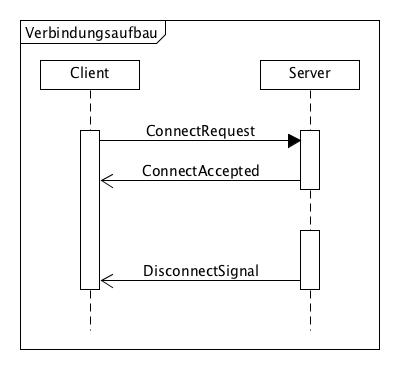
\includegraphics[height=5cm]{media/SequenceBuildConnection}
\end{center}
In dem Sequenz-Diagramm "Verbindungsaufbau"\ sieht man, wie der Verbindungsaufbau abläuft.\par
Ein Client, der sich mit dem Server verbinden möchte, schickt dem Server ein \textit{ConnectRequest} (\textbf{100}). Erhält der Client daraufhin ein \textit{ConnectAccepted} (\textbf{101}), hat sich der Client erfolgreich verbunden. Wird der \textit{ConnectRequest} abgelehnt, erhält der Client ein \textit{NotAllowed} (\textbf{920}). Das kann auftreten, wenn der Client bereits verbunden ist und schon eine \textit{ClientID} besitzt. (siehe Abschnitt \ref{sec:fehlerbehandlung} \nameref{sec:fehlerbehandlung})\par
Verlässt ein erfolgreich verbundener Client den Socket des Servers, ist das gleichbedeutend mit einem Disconnect. Ein Wiederherstellen dieser Sitzung ist nicht möglich. Er muss sich erneut mit \textit{ConnectRequest} verbinden. Ist ein Client disconnected, informiert der Server alle noch verbundenen Clients darüber mittels einem \textit{DisconnectSignal} (\textbf{200}).

\subsection{Einem Spiel beitreten \& Ingame Chat}
\begin{center}
	\begin{tabular}{| l | l | p{2.5cm} | p{2.5cm} | p{6cm} |}
		\hline
			ID & Pseudoname & Sender & Empfänger & Aktion \\
		\hline \hline
			300 & GameListRequest & Client & Server &
			Der Client fordert alle Spiele an, die bald starten, schon gestartet wurden oder vor
			Kurzem beendet wurden. \\
		\hline
			301 & GameListResponse & Server & Client &
			Der Server antwortet auf \textit{GameListRequest} (\textbf{300}) und sendet alle Spiele, die bald starten,
			schon gestartet wurden oder vor Kurzem beendet wurden. \\
		\hline
			302 & GameJoinRequest & Spieler & Server &
			Teilt dem Server mit, dass der Spieler einem Spiel als Spieler beitreten möchte. \\
		\hline
			303 & GameJoinAccepted & Server & Spieler &
			Der Server antwortet auf  \textit{GameJoinRequest} (\textbf{302}) und teilt mit, dass der Spieler dem Spiel beigetreten ist. \\
		\hline
			304 & SpectatorJoinRequest & Client & Server &
			Teilt dem Server mit, dass der Client einem Spiel als Beobachter beitreten möchte. \\
		\hline
			305 & SpectatorJoinAccepted & Server & Client &
			Der Server antwortet auf  \textit{SpectatorJoinRequest} (\textbf{304}) und teilt mit, dass der Client dem Spiel beigetreten ist. \\
		\hline
			306 & MessageSend & Client & Server &
			Sendet eine Chat-Nachricht an den Server. \\
		\hline
			307 & MessageSignal & Server & berechtigte Clients &
			Sendet eine neue Chat-Nachricht an Clients, die diese Nachricht sehen dürfen. \\
		\hline
	\end{tabular}

	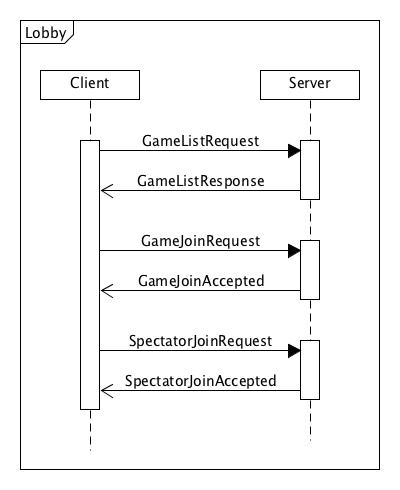
\includegraphics[height=10cm]{media/SequenceLobby}
\end{center}
In dem Sequenz-Diagramm "Lobby"\ sieht man, welche Möglichkeiten ein Client nach dem Verbinden hat.\par
Ein Client kann mittels \textit{GameListRequest} (\textbf{300}) alle existierende Spiele anfragen. Der Server antwortet darauf mit einer \textit{GameListResponse} (\textbf{301}). Die \textit{GameListResponse} umfasst eine ausführliche Liste aller Spiele. (siehe \textit{Game} in Abschnitt \ref{sec:implementierung} \nameref{sec:implementierung}).\par
Mit \textit{GameJoinRequest} (\textbf{302}) und \textit{SpectatorJoinRequest} (\textbf{304}) kann ein Client einem Spiel als Spieler, bzw. Beobachter beitreten. Erhält der Spieler danach ein \textit{GameJoinAccepted} (\textbf{303}), bzw. \textit{SpectatorJoinAccepted} (\textbf{305}) ist er erfolgreich dem Spiel beigetreten. Wird ein \textit{JoinRequest} vom Server abgelehnt, schickt er dem Client ein \textit{NotAllowed} (\textbf{920}) (siehe Abschnitt \ref{sec:fehlerbehandlung} \nameref{sec:fehlerbehandlung})\par
Zusätzlich kann der Server jederzeit ein \textit{GameJoinAccepted} (\textbf{303}) oder \textit{SpectatorJoinAccepted} (\textbf{305}) an Clients in der Lobby schicken. Wenn ein Client ein \textit{JoinAccepted} erhält, ohne ein \textit{JoinRequest} verschickt zu haben, wurde der Client vom Server zu einem Spiel hinzugefügt.\par

\newpage
\begin{center}
	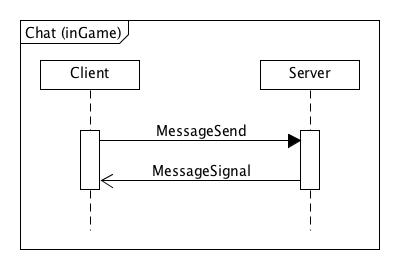
\includegraphics[width=5cm]{media/SequenceChat}\hspace{2cm}
	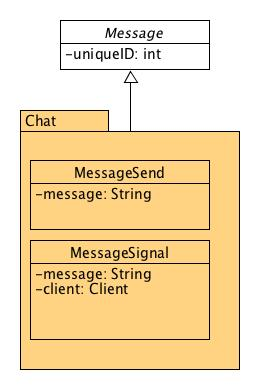
\includegraphics[width=5cm]{media/ClassChat}\\
\end{center}
Zusätzlich unterstützt jeder Server und Client eine Chatfunktion in einem Spiel. Ein Client kann mittels \textit{MessageSend} (\textbf{306}) eine Chat-Nachricht an den Server schicken. Erhält der Server ein \textit{MessageSend} prüft er den Status des Clients und wählt eine der folgenden Reaktionen:
\begin{itemize}
	\item Client ist Spieler in einem Spiel. Server sendet \textit{MessageSignal} (\textbf{307}) an alle Spieler und Beobachter in diesem Spiel.
	\item Client ist Beobachter in einem Spiel. Server sendet \textit{MessageSignal} (\textbf{307}) an alle Beobachter in diesem Spiel.
\end{itemize}

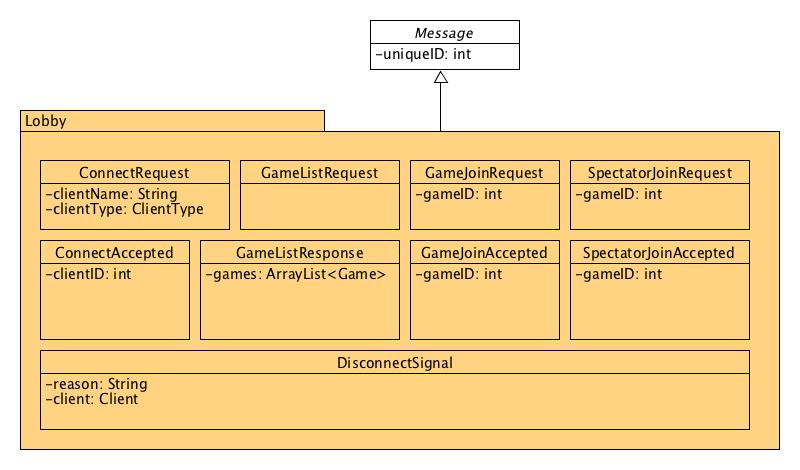
\includegraphics[width=\textwidth]{media/ClassLobby}\par
Das hier zu sehende Klassendiagramm "Lobby"\ zeigt alle Nachrichten im Detail. Zusätzlich zu den IDs und den Beschreibungen weiter oben, sieht man hier die einzelnen Klassen und ihre Attribute.\par

\newpage
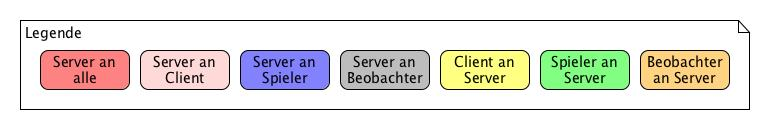
\includegraphics[width=0.8\textwidth]{media/Legend}\par
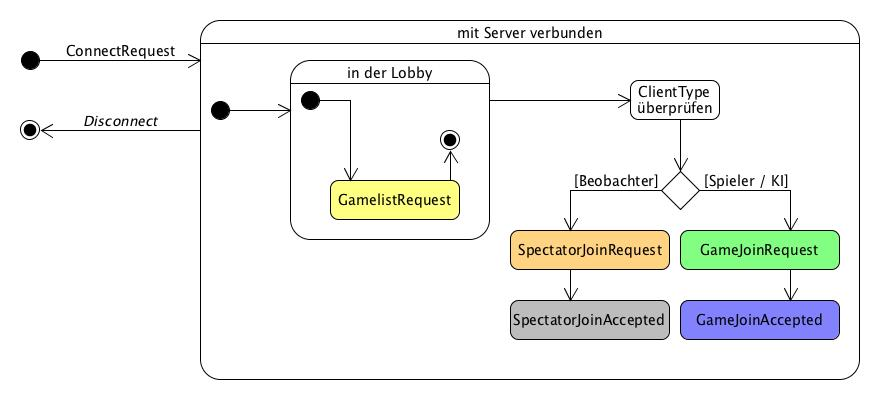
\includegraphics[width=\textwidth]{media/StateMachineConnectionAndLobby}\par
In diesem State-Chart ist der Ablauf in der Lobby noch einmal formal festgehalten.\par

\newpage
\subsection{Spiellogik}
\begin{center}
	\begin{tabular}{| l | l | p{2.5cm} | p{2.5cm} | p{6cm} |}
		\hline
			ID & Pseudoname & Sender & Empfänger & Aktion \\
		\hline \hline
			400 & StartGame & Server & Alle Clients &
			Benachrichtigt über den Spielstart und sendet die Konfiguration sowie eine Liste aller Spieler an alle Clients.\\
		\hline
			401 & EndGame & Server & Alle Clients &
			Benachrichtigt über das reguläre Ende des Spiels, welches herkömmlich durch den Sieg eines Spielers
			hervorgerufen wird oder dadurch eintritt, dass nur noch ein Spieler am Spiel beteiligt ist. \\
		\hline
			402 & AbortGame & Server & Alle Clients &
			Benachrichtigt über den Abbruch des Spiels, der durch den Ausrichter herbeigeführt wurde. \\
		\hline
			403 & PauseGame & Server & Alle Clients &
			Benachrichtigt darüber, dass der Ausrichter das Spiel pausiert hat. \\
		\hline
			404 & ResumeGame & Server & Alle Clients &
			Benachrichtigt darüber, dass der Ausrichter das Spiel fortsetzt. \\
		\hline
			405 & LeavingRequest & Client & Server &
			Teilt dem Server mit, dass der Client das Spiel verlässt. \\
		\hline
			406 & LeavingPlayer & Server & Alle Clients &
			Teilt mit, dass ein Spieler das Spiel verlassen hat. \\
		\hline
			407 & Winner & Server & Alle Clients &
			Teilt allen Clients dieses Spiels den Gewinner des Spiels und die Punkte aller Spieler mit. \\
		\hline
			408 & StartTiles & Server & Spieler &
			Sendet dem Spieler die erste Spielhand mit der konfigurierten Anzahl an Spielsteinen. \\
		\hline
			409 & CurrentPlayer & Server & Alle Clients &
			Teilt mit, welcher Spieler am Zug ist. \\
		\hline
			410 & SendTiles & Server & Spieler &
			Füllt die Hand des Spielers mit Steinen aus dem Bag. \\
		\hline
			411 & TileSwapRequest & Spieler & Server &
			Der Spieler sendet dem Server eigene Steine, die er tauschen möchte. \\
		\hline
			412 & TileSwapValid & Server & Spieler &
			Der Server teilt dem Spieler mit, ob ein \textit{TileSwapRequest} (\textbf{411}) einem gültigen Zug entspricht.\\
		\hline
			413 & TileSwapResponse & Server & Spieler &
			Der Server tauscht die Steine eines \textit{TileSwapRequest} (\textbf{411}) ein und sendet dem Spieler
			neue Steine. \\
		\hline
	\end{tabular}
\end{center}
\newpage
\begin{center}
	\begin{tabular}{| l | l | p{2.5cm} | p{2.5cm} | p{6cm} |}
		\hline
			ID & Pseudoname & Sender & Empfänger & Aktion \\
		\hline \hline
			414 & PlayTiles & Spieler & Server &
			Der Spieler teilt dem Server mit, welche Steine er wohin legen möchte. \\
		\hline
			415 & MoveValid & Server & Spieler &
			Der Server teilt dem Spieler mit, ob ein \textit{PlayTiles} (\textbf{414}) einem gültigen Zug entspricht.\\
		\hline
			416 & Update & Server & Alle Clients &
			Der Server teilt mit, welche Steine an welcher Position neu auf das Spielbrett gekommen sind. \\
		\hline
			417 & ScoreRequest & Client & Server &
			Sendet eine Anfrage nach den Scores an den Server. \\
		\hline
			418 & ScoreResponse & Server & Client &
			Antwortet auf \textit{ScoreRequest} (\textbf{417}) und sendet die Scores. \\
		\hline
			419 & TurnTimeLeftRequest & Client & Server &
			Sendet eine Anfrage nach der verbleibenden Zeit für den aktuellen Zug an den Server. \\
		\hline
			420 & TurnTimeLeftResponse & Server & Client &
			Antwortet auf \textit{TurnTimeLeftRequest} (\textbf{419}) und sendet die verbleibende Zeit in Millisekunden für den aktuellen Spielzug. \\
		\hline
			421 & TotalTimeRequest & Client & Server &
			Sendet eine Anfrage nach der Gesamtlaufzeit der Partie. \\
		\hline
			422 & TotalTimeResponse & Server & Client &
			Antwortet auf \textit{TotalTimeRequest} (\textbf{421}) und sendet die Gesamtlaufzeit der Partie in Millisekunden. \\
		\hline
			423 & BagRequest & Beobachter & Server &
			Sendet eine Anfrage nach dem Beutelinhalt. \\
		\hline
			424 & BagResponse & Server & Beobachter &
			Antwortet auf \textit{BagRequest} (\textbf{423}) und sendet den Inhalt des Beutels. \\
		\hline
			425 & PlayerHandsRequest & Beobachter & Server &
			Sendet eine Anfrage nach den Steinen, die alle Spieler auf der Hand haben. \\
		\hline
			426 & PlayerHandsResponse & Server & Beobachter &
			Antwortet auf \textit{PlayerHandsRequest} (\textbf{425}) und sendet die Steine aller Spieler. \\
		\hline
			498 & GameDataRequest & Client & Server &
			Der Client fordert den gesamten Spielzustand an. \\
		\hline
			499 & GameDataResponse & Server & Client &
			Der Server sendet den gesamten Spielzustand. \\
		\hline
	\end{tabular}
\end{center}

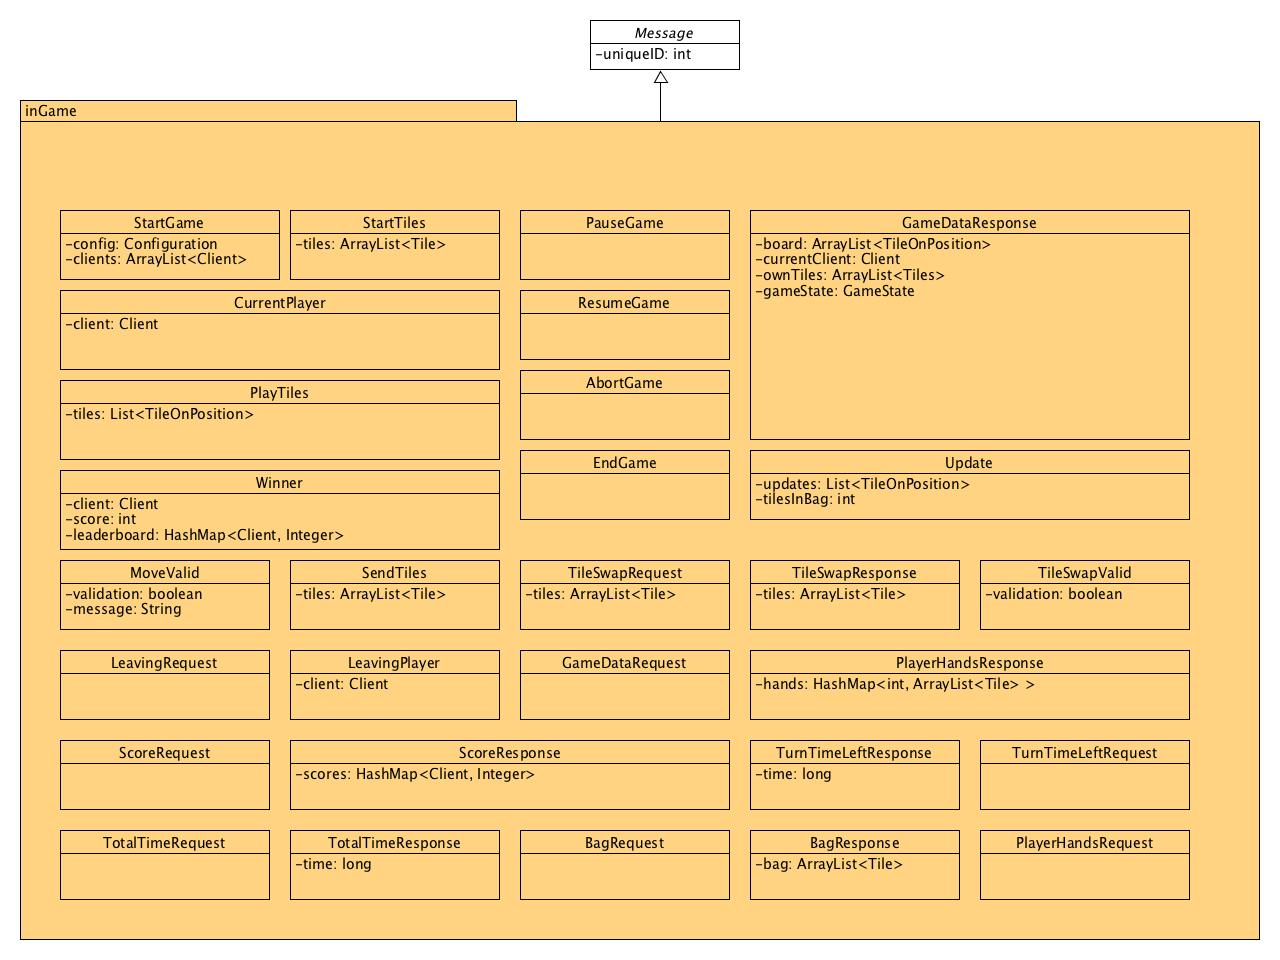
\includegraphics[width=\textwidth]{media/ClassInGame}\par
Das hier zusehende Klassendiagramm "{InGame}"\ zeigt alle Nachrichten im Detail. Zusätzlich zu den IDs und den Beschreibungen weiter oben, sieht man hier die einzelnen Klassen und ihre Attribute.\par

\newpage
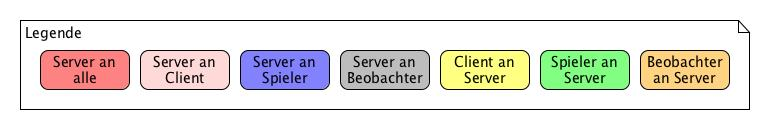
\includegraphics[width=0.8\textwidth]{media/Legend}\par
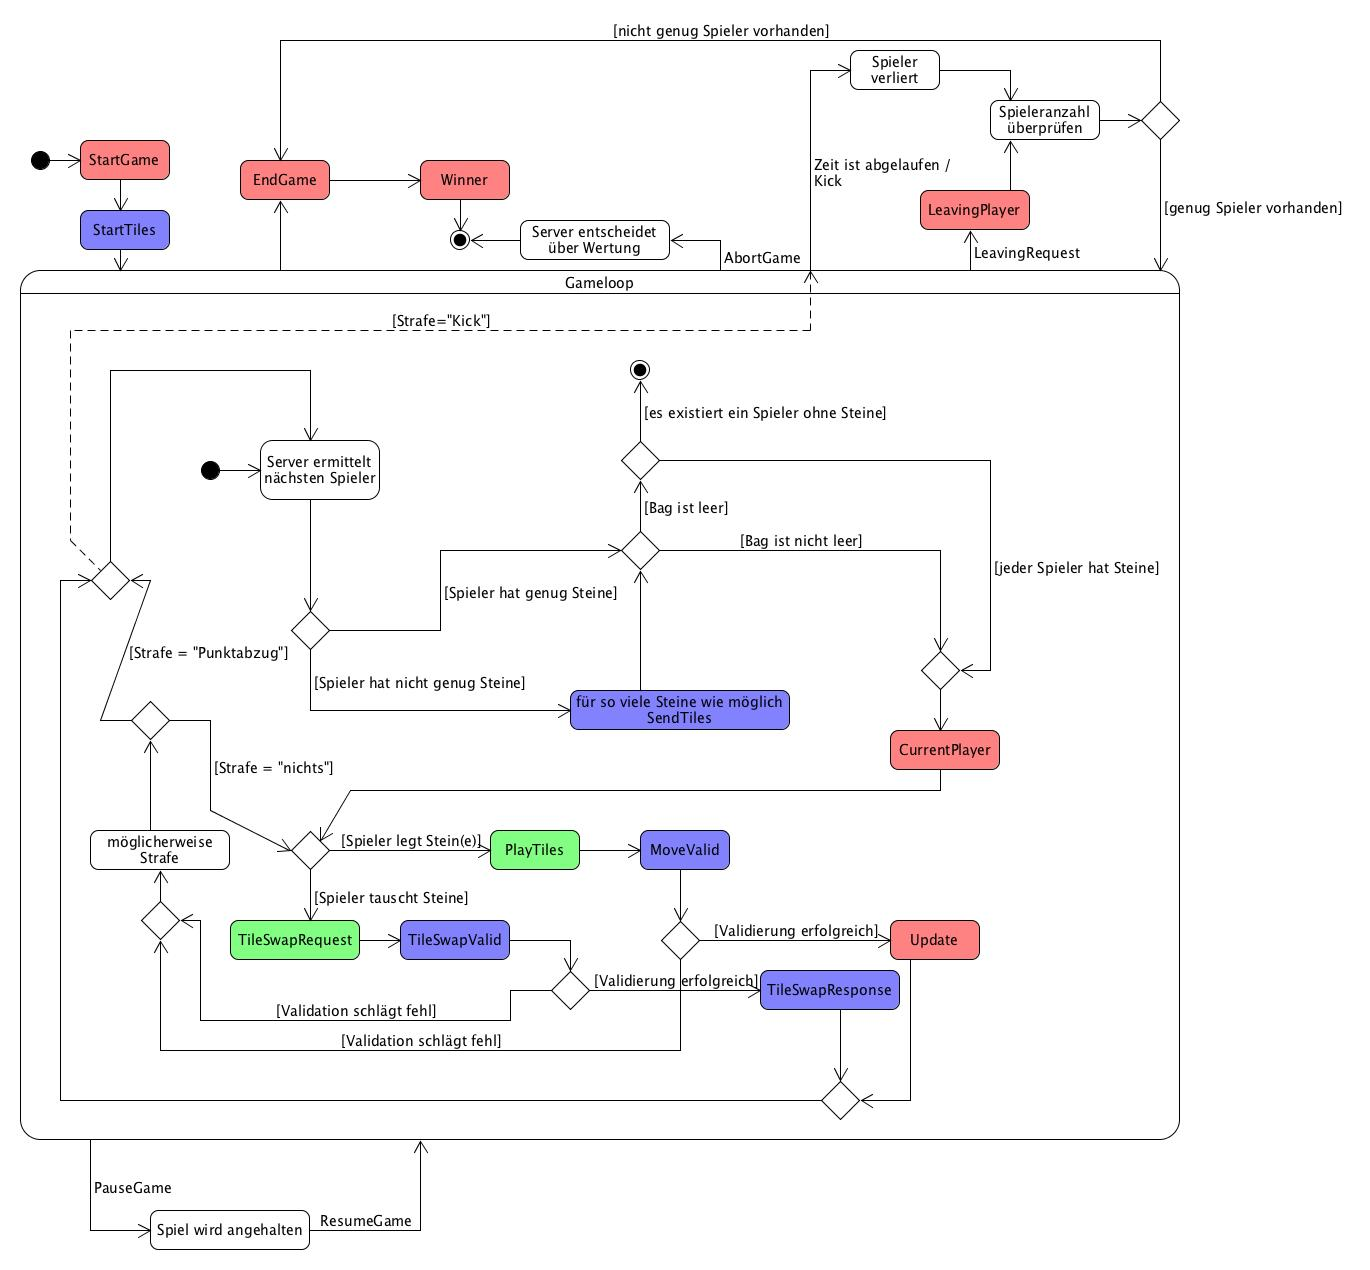
\includegraphics[width=\textwidth]{media/StateMachineGame}\par
In diesem State-Chart wird das Verhalten in einer Spielsitzung beschrieben. Wir beschreiben hier nur Eigenschaften, die nicht eindeutig aus dem State-Chart erkennbar sind.\par
Wird ein Spiel vom Ausrichter gestartet, wird vom Ausrichter eine Reihenfolge der Spieler gewählt, nach dieser sind die Spieler pro Runde am Zug.\par
In jedem Spiel muss beim ersten \textit{PlayTiles} (\textbf{414}) genau einen Stein die Koordinaten $(x, y)=(0, 0)$ haben. Ansonsten ist der Zug nicht valide und der Server sendet dem Client  \textit{MoveValid} (\textbf{415}) mit \textit{validation=false}.\par
Die Zugzeit eines Spielers beginnt, nachdem vom Server \textit{CurrentPlayer} (\textbf{409}) an alle Clients in diesem Spiel verschickt wurde. Der Spieler muss innerhalb seiner Zugzeit einen validen Zug mit \textit{PlayTiles} (\textbf{414}) oder \textit{TileSwapRequest} (\textbf{411}) an den Server verschicken.\par
Ob ein \textit{TileSwapRequest} (\textbf{411}) valide ist, wird vom Server geprüft. Der Client erhält die Antwort mittels \textit{TileSwapValid} (\textbf{412}). Ein \textit{TileSwapRequest} ist nicht valide, wenn der Client mehr Steine anfordert, als er auf der Hand hat oder noch im Bag sind.\par
Alle Antworten auf \textit{Request}-Anfragen basieren auf dem Stand der bereits per \textit{CurrentPlayer} (\textbf{409}) oder \textit{Update} (\textbf{416}) an alle Clients verschickt wurde. Auch wenn der Server schon einen aktuelleren Stand hat.\\
Beispiel: Spieler A schickt validen Zug an Server und hat ein \textit{MoveValid} erhalten. Nun fragt Beobachter B mit \textit{GameDataRequest} die Spieldaten ab. Wird die \textit{GameDataResponse} vor dem \textit{Update} verschickt, ist der Zug von Spieler A noch nicht darin enthalten.\par
Fragt ein Beobachter mit \textit{GameDataRequest} (\textbf{498}) die Spieldaten ab, ist \textit{OwnTiles} eine leere Liste.\par
Wird ein Spieler aus einem Spiel gekickt oder disconnected, entfällt er aus der Wertung, seine Steine auf der Hand werden in den Bag zurückgegeben und die Steine auf dem Spielfeld bleiben liegen.\par

\subsection{Erläuterung der Implementierung}
\label{sec:implementierung}
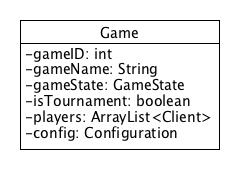
\includegraphics[width=5cm]{media/ClassGame}
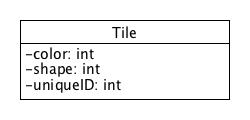
\includegraphics[width=5cm]{media/ClassTile}
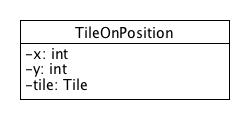
\includegraphics[width=5cm]{media/ClassTileOnPosition}
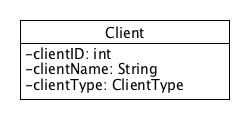
\includegraphics[width=5cm]{media/ClassClient}
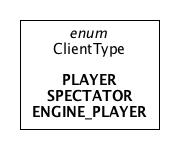
\includegraphics[width=2.5cm]{media/EnumClientType}
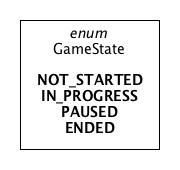
\includegraphics[width=2.5cm]{media/EnumGameState}
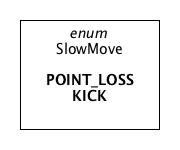
\includegraphics[width=2.5cm]{media/EnumSlowMove}
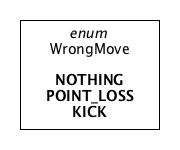
\includegraphics[width=2.5cm]{media/EnumWrongMove}\par

Diese Klassen werden vom Interface-Komitee bereitgestellt. Sie werden in einigen Message-Klassen benutzt, um Informationen strukturiert zu übermitteln.\par

\begin{center}
    \begin{tabular}{| l | l | p{4.2cm} | p{6cm} |}
        \hline
            ID & Pseudoname & Attribute & Erklärung \\
        \hline \hline
            100 & ConnectRequest & String \textit{clientName} & Name des Spielers \\
        \cdashline{3-4}
        	& & ClientType \textit{clientType} & Typ des Clients \\
        \hline
            101 & ConnectAccepted & int \textit{clientID} & interne ID des Spielers \\
        \hline
        	200 & DisconnectSignal & String \textit{reason} & Begründung \\
        \cdashline{3-4}
        	& & Client \textit{client} & Klasse des getrennten Clients \\
        \hline
        	300 & GameListRequest & & \\
        \hline
        	301 & GameListResponse & ArrayList<Game> \textit{games} & Liste aller Spiele \\
        \hline
        	302 & GameJoinRequest & int \textit{gameID} & ID des Spiels \\
        \hline
        	303 & GameJoinAccepted & int \textit{gameID} & ID des Spiels \\
        \hline
        	304 & SpectatorJoinRequest & int \textit{gameID} & ID des Spiels \\
        \hline
        	305 & SpectatorJoinAccepted & int \textit{gameID} & ID des Spiels \\
        \hline
        	306 & MessageSend & String \textit{message} & Die zu übertragene Chat-Nachricht \\
        \hline
        	307 & MessageSignal & String \textit{message} & Die neue Chat-Nachricht \\
        \cdashline{3-4}
        	& & Client \textit{client} & Klasse des Clients, der die Nachricht verschickt hat \\
        \hline
        \end{tabular}
       \begin{tabular}{| l | l | p{4.2cm} | p{6cm} |}
	   \hline
            ID & Pseudoname & Attribute & Erklärung \\
        \hline \hline

        	400 & StartGame & Configuration \textit{config} & Spielkonfiguration \\
        \cdashline{3-4}
        	& & ArrayList<Client> \textit{clients} & Liste aller Spieler \\
        \hline
        	401 & EndGame & & \\
        \hline
        	402 & AbortGame & & \\
        \hline
        	403 & PauseGame & & \\
        \hline
        	404 & ResumeGame & & \\
        \hline
        	405 & LeavingRequest & & \\
        \hline
        	406 & LeavingPlayer & Client \textit{client} & Client, der das Spiel verlassen hat \\
        \hline
        	407 & Winner & Client \textit{client} & Client, der gewonnen hat \\
        \cdashline{3-4}
        	& & int \textit{score} & Punkte des Gewinners \\
        \cdashline{3-4}
        	& & HashMap<Client, Integer> \textit{leaderboard} & Auflistung aller Spieler (als Key) und der jeweiligen Punktzahl (als Value) \\
        \hline
        	408 & StartTiles & ArrayList<Tile> \textit{tiles} & Liste aller Steine, die der Spieler zu Beginn bekommt \\
        \hline
        	409 & CurrentPlayer & Client \textit{client} & Client, der gerade am Zug ist \\
        \hline
        	410 & SendTiles & ArrayList<Tile> \textit{tiles} & Liste der Steine, die ein Spieler aus dem Bag bekommt \\
        \hline
        	411 & TileSwapRequest & ArrayList<Tile> \textit{tiles} & Liste der Steine, die der Spieler tauschen möchte \\
        \hline
        	412 & TileSwapValid & boolean \textit{validation} & Dürfen die Steine getauscht werden? \\
        \hline
        	413 & TileSwapResponse & ArrayList<Tile> \textit{tiles} & Liste der Steine, die der Spieler durch einen Tausch erhält \\
        \hline
        	414 & PlayTiles & ArrayList<TileOnPosition> \textit{tiles} & Liste der Steine, die der Spieler legen will sowie deren Position auf dem Spielfeld \\
        \hline
        	415 & MoveValid & boolean \textit{validation} & Dürfen die Steine so gelegt werden? \\
        \cdashline{3-4}
        	& & String \textit{message} & Begründung \\
        \hline
        	416 & Update & ArrayList<TileOnPosition> \textit{updates} & Liste aller Steine, die im letzten Spielzug auf das Brett gelegt wurden sowie deren Position auf dem Brett \\
        \hline
        	417 & ScoreRequest & & \\
        \hline
        	418 & ScoreResponse & HashMap<Client, Integer> \textit{scores} & Auflistung aller Spieler (als Key) und des jeweiligen Punktestands (als Value) \\
        \hline
        	419 & TurnTimeLeftRequest & & \\
        \hline
        	420 & TurnTimeLeftResponse & long \textit{time} & Die restliche Zeit für den aktuellen Spielzug \\
        \hline
        	421 & TotalTimeRequest & & \\
        \hline
        	422 & TotalTimeResponse & long \textit{time} & Zeit, die bisher im gesamten Spiel verstrichen ist \\
        \hline
        	423 & BagRequest & & \\
        \hline
        	424 & BagResponse & ArrayList<Tile> \textit{bag} & Liste aller Steine im Beutel \\
        \hline
        	425 & PlayerHandsRequest & & \\
        \hline
        	426 & PlayerHandsResponse & HashMap<Client, ArrayList<Tile> > \textit{hands} & Auflistung aller Spieler (als Key) und jeweils einer Liste der Handsteine des Spielers (als Value) \\
        \hline
        	498 & GameDataRequest & & \\
        \hline
        	499 & GameDataResponse & List<TileOnPosition> \textit{board} & Liste aller auf dem Brett liegenden Steine sowie deren Position \\
        \cdashline{3-4}
        	& & Client \textit{currentClient} & Die ID des Spielers, der gerade am Zug ist \\
        \cdashline{3-4}
        	& & List<Tile> \textit{ownTiles} & Liste aller Steine, die der Spieler auf der Hand hat (leere Liste, wenn von Beobachter angefragt) \\
        \cdashline{3-4}
        	& & boolean \textit{paused} & Ist das Spiel pausiert? \\
        \hline
    \end{tabular}

    \begin{tabular}{| l | p{4cm} | p{6cm} |}
	\hline
          Klasse & Attribute / \textbf{Instanzen} & Erklärung \\
        \hline \hline
        	ClientType & \textbf{PLAYER} & Der Client ist ein aktiver Spieler.\\
        \cdashline{2-3}
        	\textbf{enum} & \textbf{SPECTATOR} & Der Client ist ein Beobachter \\
        \cdashline{2-3}
		 & \textbf{ENGINE\_PLAYER} & Der Client ist ein AI-Teilnehmer \\
        \hline
        WrongMove & \textbf{NOTHING} & Der Spieler ist erneut an der Reihe \\
       \cdashline{2-3}
       	\textbf{enum} & \textbf{POINT\_LOSS} & Der Spieler erhält die konfigurierte Anzahl an Strafpunkten und der nächste Spieler ist an der Reihe \\
       \cdashline{2-3}
       	& \textbf{KICK} & Der Spieler wird vom Spiel ausgeschlossen und der nächste Spieler ist an der Reihe \\
       \hline
       SlowMove & \textbf{POINT\_LOSS} & Der Spieler erhält die konfigurierte Anzahl an Strafpunkten und der nächste Spieler ist an der Reihe\\
       \cdashline{2-3}
       	\textbf{enum} & \textbf{KICK} & Der Spieler wird vom Spiel ausgeschlossen und der nächste Spieler ist an der Reihe \\
       \hline
        GameState & \textbf{NOT\_STARTED} & Das Spiel ist noch nicht gestartet \\
       \cdashline{2-3}
       	\textbf{enum} & \textbf{IN\_PROGRESS} & Das Spiel läuft \\
       \cdashline{2-3}
       	& \textbf{PAUSED} & Das Spiel ist pausiert \\
       	\cdashline{2-3}
       	& \textbf{ENDED} & Das Spiel ist beendet \\
       \hline
        	Configuration & int \textit{colorShapeCount} & Anzahl der Farben bzw. der Symbole \\
        \cdashline{2-3}
        	& int \textit{tileCount} & Häufigkeit eines Spielsteins \\
        \cdashline{2-3}
        	& int \textit{maxHandTiles} & Anzahl der Steine, die man auf der Hand haben darf \\
        \cdashline{2-3}
        	& long \textit{turnTime} & Zeit für jeden Zug \\
        \cdashline{2-3}
        	& long \textit{timeVisualization} & Zeit für die Visualisierung des letzten Zugs \\
        \cdashline{2-3}
        	& WrongMove \textit{wrongMove} & Strafe für fehlerhaften Zug \\
        \cdashline{2-3}
        	& int \textit{wrongMovePenalty} & Strafpunkte für einen fehlerhaften Zug \\
        \cdashline{2-3}
        	& SlowMove \textit{slowMove} & Strafe für Ablauf der Zugzeit \\
        \cdashline{2-3}
        	& int \textit{slowMovePenalty} & Strafpunkte für Ablauf der Zugzeit \\
		\cdashline{2-3}
        	& int \textit{maxPlayerNumber} & maximale Spieleranzahl für das Spiel \\
        \hline
        	Client & int \textit{clientID} & ID des Clients \\
        \cdashline{2-3}
         & String \textit{clientName} & Name des Client \\
        \cdashline{2-3}
        	& ClientType \textit{clientType} & Typ des Clienten \\
        \hline
        	Game & int \textit{gameID} & ID des Spiels \\
        \cdashline{2-3}
        	& String \textit{gameName} & Name des Spiels \\
        \cdashline{2-3}
        	& GameState \textit{gameState} & Status des Spiels \\
        \cdashline{2-3}
        	& boolean \textit{isTournament} & Gehört das Spiel zu einem Turnier? \\
        \cdashline{2-3}
        	& ArrayList<Client> \textit{players} & Liste der Spieler des Spiels \\
        \cdashline{2-3}
        	& Configuration \textit{config} & Spielkonfiguration \\
        \hline
        	Tile & int \textit{color} & Farbe des Spielsteins \\
        \cdashline{2-3}
        	& int \textit{shape} & Symbol des Spielsteins \\
        \cdashline{2-3}
        	& int \textit{uniqueID} & einzigartige ID zur eindeutigen Identifizierung jedes Steins \\
        \hline
        TileOnPosition & int \textit{x} & x-Koordinate des Steins \\
       \cdashline{2-3}
       	& int \textit{y} & y-Koordinate des Steins \\
       \cdashline{2-3}
       	& Tile \textit{tile} & Der Spielstein zu den Koordinaten \\
       \hline


    \end{tabular}

\end{center}

\newpage
\section{Fehlerbehandlung}
\label{sec:fehlerbehandlung}
Bei der Kommunikation zwischen Client und Server können viele verschiedene Fehler auftreten.
Ein Fehler enthält eine Nachricht und ist genau einer der drei Typen: AccessDenied, ParsingError oder NotAllowed. Fehler werden ebenfalls als Message-Objekt vom Server an den jeweiligen Client gesendet.

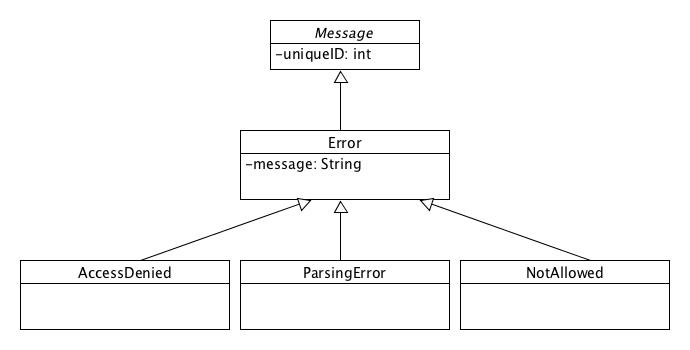
\includegraphics[width=\textwidth]{media/ClassError}

In der folgenden Tabelle wird kurz erklärt in welchen Situationen die jeweiligen Fehlertypen vorkommen.
\begin{center}
	\begin{tabular}{| l | l | p{2.5cm} | p{2.5cm} | p{6cm} |}
		\hline
			ID & Pseudoname & Sender & Empfänger & Erklärung \\
		\hline \hline
			900 & AccessDenied & Server & Client&
			Der Client hat nicht die nötigen Rechte um diese Nachricht zu senden. \\
		\hline
			910 & ParsingError & Server & Client &
			Die zuletzt gesendete Nachricht konnte nicht korrekt interpretiert werden.\\
		\hline
			920 & NotAllowed & Server & Client &
            Die Nachricht ist im aktuellen Zustand nicht zulässsig. \\
		\hline
	\end{tabular}
\end{center}

\newpage
Die folgende Tabelle stellt dar, zu welchen Nachrichten welche Fehler auftreten können und welche Nachrichtensender dies betrifft. Sollten mehrere Fehler auftreten wird immer der Fehler mit der höchsten Priorität zurückgesendet.
Die Prioritäten sind: ParsingError > AccessDenied > NotAllowed. \\

\begin{center}
	\begin{tabular}{| l | l | l | l |}
		\hline
			ID & Rolle & Beschreibung & Fehlermeldung\\
		\hline \hline
			alle & - & Nachricht konnte nicht korrekt interpretiert werden. & ParsingError\\
		\hline
			100 & Client &
			Client ist schon verbunden. & NotAllowed\\
		\hline
			300 & Client &
			Client ist schon in einem Spiel. & NotAllowed\\
		\hline
			302 & Spieler &
			Spieler ist schon in einem Spiel. & NotAllowed\\
		\hline
			302 & Spieler & Das Spiel hat schon angefangen. & NotAllowed\\
		\hline
			302 & Beobachter &
			Keine Berechtigung für Beobachter. & AccessDenied\\
		\hline
			304 & Client &
			Client beobachtet oder spielt schon. & NotAllowed\\
		\hline
			306 & Client &
			Client nicht im Spiel. & NotAllowed\\
		\hline
			405 & Client &
			Client nicht im Spiel. & NotAllowed\\
		\hline
			411 & Spieler & Spieler ist nicht am Zug. & NotAllowed\\
		\hline
			411 & Beobachter & Keine Berechtigung als Beobachter. & AccessDenied\\
		\hline
			414 & Spieler & Spieler ist nicht am Zug. & NotAllowed\\
		\hline
			414 & Spieler & Der Stein ist nicht bekannt. & ParsingError\\
		\hline
			414 & Beobachter & Keine Berechtigung als Beobachter. & AccessDenied\\
		\hline
			417 & Client & Client nicht im Spiel. & NotAllowed\\
		\hline
			419 & Client & Client nicht im Spiel. & NotAllowed\\
		\hline
			421 & Client & Client nicht im Spiel. & NotAllowed\\
		\hline
			423 & Client & Client nicht im Spiel. & NotAllowed\\
		\hline
			423 & Spieler & Keine Berechtigung als Spieler. & AccessDenied\\
		\hline
			425 & Beobachter & Beobachter nicht im Spiel. & NotAllowed\\
		\hline
			425 & Spieler & Keine Berechtigung als Spieler. & AccessDenied\\
		\hline
			498 & Client & Client nicht im Spiel. & NotAllowed\\
		\hline
	\end{tabular}
\end{center}

\newpage
\section{Konfiguration}
\label{sec:konfiguration}
\begin{center}
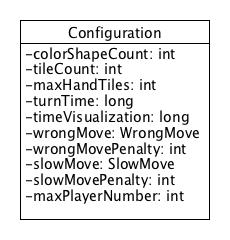
\includegraphics[width=4cm]{media/ClassConfiguration}
\end{center}
Die Konfiguration wird gespeichert, indem die Configuration Klasse serialisiert in einer .json Datei gespeichert wird. \par
In der Konfiguration besteht die Option slowMove als KICK oder POINT\_LOSS festzulegen. Diese Option definiert, wie sich der Server bei abgelaufender Zugzeit verhält. \\
Die Option wrongMove erlaubt: KICK, POINT\_LOSS, NOTHING. Diese Option tritt bei regelwidrigen Zügen in Kraft. \\
Die Anzahl der abgezogenen Punkte lässt sich unter der Option penalty konfigurieren. \\
Die Optionen KICK, POINT\_LOSS und NOTHING bewirken folgendes:
\begin{itemize}
	\item KICK: Verbindung zum Server wird vom Server getrennt.
	\item POINT\_LOSS: Die in penalty definierte Anzahl an Punkten wird vom Punktekonto des Spielers subtrahiert.
	\item NOTHING: Der Spieler bekommt keine Strafe und darf in seiner verbleibenden Zugzeit einen neuen Zug machen.
\end{itemize}
Mit der Option maxPlayerNumber wird bestimmt, wie viele Spieler in diesem Spiel sein dürfen. Ist die maximale Spieleranzahl mit 0 in der Konfiguration angegeben, bedeutet dies das keine Spielerobergrenze definiert ist. Die minimale Spieleranzahl muss immer mindestens 2 sein.
ColorShapeCount ist 0 basiert.

\section{Changelog}
\label{sec:changelog}
\begin{center}
	\begin{tabular}{| p{2cm} | p{12cm} |}
	\hline
		Version 1.0.1 & Rechtschreibfehler behoben, Erläuterungen im Dokument hinzugefügt, \newline
		Implementierung optimiert (ohne Änderung der API).\\
	\hline
	\end{tabular}

\end{center}

\end{document}
